\documentclass{mc2015}
%
%=================================================================================================
% new commands
% +++++++++++++++++++++++++++++++++++++++++++++++++++++++++++++++++++++++++++++++++++++++++++++++++
\newcommand{\nc}{\newcommand}

\renewcommand{\div}{\mbold{\nabla}\! \cdot \!}
\newcommand{\grad}{\mbold{\nabla}}
\newcommand{\divv}[1]{\boldsymbol{\nabla}^{#1}\! \cdot \!}
\newcommand{\gradd}[1]{\mbold{\nabla}^{#1}}
\newcommand{\mbold}[1]{\boldsymbol#1}
% latex shortcuts
\newcommand{\bea}{\begin{eqnarray}}
\newcommand{\eea}{\end{eqnarray}}
\newcommand{\be}{\begin{equation}}
\newcommand{\ee}{\end{equation}}
\newcommand{\bal}{\begin{align}}
\newcommand{\eali}{\end{align}}
\newcommand{\bi}{\begin{itemize}}
\newcommand{\ei}{\end{itemize}}
\newcommand{\ben}{\begin{enumerate}}
\newcommand{\een}{\end{enumerate}}
\usepackage{amsthm}
\newtheorem*{remark}{Remark}
% DGFEM commands
\newcommand{\jmp}[1]{[\![#1]\!]}                     % jump
\newcommand{\mvl}[1]{\{\!\!\{#1\}\!\!\}}             % mean value
\newcommand{\keff}{\ensuremath{k_{\textit{eff}}}\xspace}
% shortcut for domain notation
\newcommand{\D}{\mathcal{D}}
% vector shortcuts
\newcommand{\vo}{\mbold{\Omega}}
\newcommand{\vr}{\mbold{r}}
\newcommand{\vn}{\mbold{n}}
\newcommand{\vnk}{\mbold{\mathbf{n}}}
\newcommand{\vj}{\mbold{J}}
\newcommand{\eig}[1]{\| #1 \|_2}
%
\newcommand{\EI}{\mathcal{E}_h^i}
\newcommand{\ED}{\mathcal{E}_h^{\partial \D^d}}
\newcommand{\EN}{\mathcal{E}_h^{\partial \D^n}}
\newcommand{\ER}{\mathcal{E}_h^{\partial \D^r}}
\newcommand{\reg}{\textit{reg}}
%
\newcommand{\norm}{\textrm{norm}}
\renewcommand{\Re}{\textrm{Re}}
\newcommand{\Pe}{\textrm{P\'e}}
\renewcommand{\Pr}{\textrm{Pr}}
%
\newcommand{\resi}{R}
%\newcommand{\resinew}{\tilde{D}_e}
\newcommand{\resinew}{\widetilde{\resi}}
\newcommand{\resisource}{\widetilde{\resi}^{source}}
\newcommand{\matder}[1]{\frac{\textrm{D} #1}{\textrm{D} t}}
%
\newcommand{\Gammakj}{\Gamma_{k \to j}}

% extra space
\newcommand{\qq}{\quad\quad}
% common reference commands
\newcommand{\eqt}[1]{Eq.~(\ref{#1})}                     % equation
\newcommand{\eqts}[1]{Eqs.~(\ref{#1})}                     % equations
\newcommand{\fig}[1]{Fig.~\ref{#1}}                      % figure
\newcommand{\tbl}[1]{Table~\ref{#1}}                     % table
\newcommand{\sct}[1]{Section~\ref{#1}}                   % section
\newcommand{\app}[1]{Appendix~\ref{#1}}                   % appendix
\newcommand{\lem}[1]{Lemma~\ref{#1}}                   % lemma
\newcommand{\theo}[1]{Theorem~\ref{#1}}                   % theorem
%
\newcommand{\ie}{i.e.,\@\xspace}
\newcommand{\eg}{e.g.,\@\xspace}
\newcommand{\psc}[1]{{\sc {#1}}}
\newcommand{\rs}{\psc{R7}\xspace}
%
\newcommand\br{\mathbf{r}}
%\newcommand{\tf}{\varphi}
\newcommand{\tf}{b}
%
%\renewcommand{\dim}{\ensuremath{\texttt{dim}}\xspace}
%
\newcommand{\tcr}[1]{\textcolor{red}{#1}}
\newcommand{\tcb}[1]{\textcolor{blue}{#1}}
  \newcommand{\tcg}[1]{\textcolor{green}{#1}}
\newcommand{\mt}[1]{\marginpar{ {\tiny #1}}}

\newtheorem{theorem}{Theorem}[section]
\newtheorem{lemma}[theorem]{Lemma}

%%%%%%%%%%%%%%%%%%%%%%%%%%%%%%%%%%%%%%%%%%%%%%%%%%%%%%%%%%%%%%%%%%%%%
\usepackage[T1]{fontenc}         % Use T1 encoding instead of OT1
\usepackage[utf8]{inputenc}      % Use UTF8 input encoding
\usepackage{microtype}           % Improve typography
\usepackage{booktabs}            % Publication quality tables
\usepackage{amsmath}
\usepackage{amssymb}
\usepackage{graphicx}
\usepackage{float}
\usepackage[exponent-product=\cdot]{siunitx}
\usepackage[colorlinks,breaklinks]{hyperref}
\hypersetup{linkcolor=black, citecolor=black, urlcolor=black}

\usepackage{lipsum}


\usepackage{color}
\usepackage{caption}
\usepackage{subcaption}
\usepackage{mathrsfs}
% more math
\usepackage{amsfonts}
\usepackage{amstext}
\usepackage{amsbsy}
\usepackage{mathbbol} 


\def\equationautorefname{Eq.}
\def\figureautorefname{Fig.}

%%%%%%%%%%%%%%%%%%%%%%%%%%%%%%%%%%%%%%%%%%%%%%%%%%%%%%%%%%%%%%%%%%%%%
% Insert authors' names and short version of title in lines below

\authorHead{Marc O. Delchini, Jean C. Ragusa, Ray A. Berry, and Richard Martineau}
\shortTitle{Water hammer simulations with RELAP-7}

%%%%%%%%%%%%%%%%%%%%%%%%%%%%%%%%%%%%%%%%%%%%%%%%%%%%%%%%%%%%%%%%%%%%%
\begin{document}

\title{Application of the reactor system code RELAP-7 to single- and two-phase flow water-hammer problems}

\author{Marc O. Delchini}
\author{Jean C. Ragusa}
\affil{
  Department of Nuclear Engineering \\
  Texas A\&M University \\
  College Station, TX 77843 \\
  delchmo@tamu.edu; jean.ragusa@tamu.edu}

\author{Ray A. Berry}
\author{Richard Martineau}
\affil{
  Idaho National Laboratory \\
	Idaho Falls, ID 83415 \\
  ray.berry@inl.gov; richard.martineau@inl.gov
}

\maketitle

\begin{abstract}
The primary basis of the RELAP-7 governing theory includes the single-phase Euler equations and the 7-equation two-phase flow models. 
It is well established that these hyperbolic conservation laws can develop shocks and discontinuities and thus, require a stabilization 
numerical method. The all-Mach flow Entropy Viscosity Method is now employed in RELAP-7 as a stabilization numerical method for both 
above flow models. The entropy viscosity technique is a viscous regularization technique: adequate dissipation terms (viscous fluxes) are 
added to the governing laws while ensuring the entropy minimum principle still holds. Viscosity coefficients modulates the magnitude of the 
added dissipation such that it is large in shock regions and vanishingly small elsewhere. The stabilization capabilities of the Entropy Viscosity 
Method are demonstrated in the system code RELAP-7 by simulating a 1-D single and two-phase water-hammers. \\
%
\emph{Key Words}:  RELAP-7 ; numerical method ; entropy viscosity method ; low-Mach flow ; shocks ; single phase flow ; two-phase flow.
\end{abstract}

%%%%%%%%%%%%%%%%%%%%%%%%%%%%%%%%%%%%%%%%%%%%%%%%%%%%%%%%%%%%%%%%%%%%%%%%%%%%%
\section{Introduction}\label{sec:intro}
%%%%%%%%%%%%%%%%%%%%%%%%%%%%%%%%%%%%%%%%%%%%%%%%%%%%%%%%%%%%%%%%%%%%%%%%%%%%%
%
Single- and tow-phase flow water hammer problems are simulated using RELAP-7 (Reactor Excursion and Leak Analysis Program),
the next-generation nuclear reactor system analysis code under development at Idaho National Laboratory (INL). 
%
Water hammer, or hydraulic shock, is a pressure surge or wave caused when a fluid in motion is forced to stop or change direction abruptly. 
In nuclear power plants, water hammers commonly occur 
in case of an inflow of sub-cooled water into pipes or other parts of the equipment, which are filled with steam or steam-water mixture; they also
happen as the consequence of valve closing or opening actions or of breaks in pipes, with single phase or two-phase flow. 
% when a valve closes suddenly at an end of a pipe system, and a pressure wave propagates in the pipe. 

The RELAP-7 code is built using modern scientific software libraries (the Multi-Physics Object Oriented Simulation Environment MOOSE \cite{MOOSE}, 
itself built upon PETSc and LibMesh, among others).  
%
The primary basis for RELAP-7's governing theory includes Euler single-phase equations \cite{Toro} and the 7-equation two-phase flow model of \cite{SEM}. 
This two-phase flow model is strictly hyperbolic, as opposed to the 6-equation model RELAP-5.  
It is well established that hyperbolic conservation laws can develop shocks and discontinuities \cite{Leveque} and, therefore, require stabilization 
of the discretized equations. Fot single-phase Euler equations, numerous numerical methods are available both for discontinuous and continuous discretization schemes 
\cite{Toro, Lapidus_paper, LMP, Lapidus_book, Roe, SUPG}. Until recently, the 7-equation model was only discretized in space using discontinuous schemes with approximate 
Riemann solvers derived using well-established approaches for single-phase flows, while using an upwind-type flux for the non-conservative terms 
\cite{Saurel_2001a, Saurel_2001b, Li_2004, Zein_2010, Ambroso_2012}. 
%
In RELAP-7, the conservation laws are discretized using a \emph{Continuous Galerkin Finite Element Method} and the resulting discrete equations are stabilized using 
the Entropy Viscosity Method \cite{jlg1, jlg2}.
%  that is independent of the type of spatial discretization (finite volume, continuous or discontinuous finite elements, ...) and thus may be applied ubiquitously.
 


The entropy viscosity technique is a viscous regularization technique where adequate dissipation terms (viscous fluxes) are added to the governing laws while ensuring 
that the entropy minimum principle holds. Viscosity coefficients modulates the magnitude of the added dissipation such that it is large in shock regions and vanishingly 
small elsewhere. The entropy viscosity coefficients are taken proportional to the entropy production while, at the same time, being bounded from above by a first-order 
viscosity coefficient that reduces the spatial discretization to be similar to a first-order Godunov scheme (the latter being known to be overly dissipative but monotone 
\cite{you had [12]). Hence, entropy production in shocks will result in large viscosity coefficients and thus will avoid spurious oscillations. In order to solve for 
low-Mach flows \cite{LowMach1, LowMach2, LowMach3}, the original version of the Entropy Viscosity Method was modified and new definitions of the viscosity coefficients 
were proposed to ensure well-scaled dissipative terms in the low-Mach asymptotic limit while preserving the capabilities of the method to resolve shocks and discontinuities 
\cite{Marco_dissertation, Marco_paper_low_mach}. The same approach was used to extend the method to the 7-equation two-phase flow model 
\cite{Marco_paper_7_equ, Marco_dissertation}. 

In this paper, the single and two-phase flow models, regularized with the entropy viscosity method, are recalled along with the all-Mach flow definitions of the viscosity coefficients 
in \sct{sct:model}. After providing the spatial and temporal discretization method in \sct{sec:disc}, numerical results of single and a two-phase water-hammer problems are 
presented in \sct{sec:results}. 

%
%%%%%%%%%%%%%%%%%%%%%%%%%%%%%%%%%%%%%%%%%%%%%%%%%%%%%%%%%%%%%%%%%%%%%%%%%%%%%
%%%%%%%%%%%%%%%%%%%%%%%%%%%%%%%%%%%%%%%%%%%%%%%%%%%%%%%%%%%%%%%%%%%%%%%%%%%%%
\section{Single phase and two-phase flow models}\label{sct:model}
%%%%%%%%%%%%%%%%%%%%%%%%%%%%%%%%%%%%%%%%%%%%%%%%%%%%%%%%%%%%%%%%%%%%%%%%%%%%%
%%%%%%%%%%%%%%%%%%%%%%%%%%%%%%%%%%%%%%%%%%%%%%%%%%%%%%%%%%%%%%%%%%%%%%%%%%%%%
%
In this section, the single- and the two-phase flow models implemented in RELAP-7 are recalled, along with their viscous regularization via the entropy viscosity method 
and the definition of the viscosity coefficients that are appropriate for all-Mach flows. % definition of used in the application of the numerical method called the Method (EVM). 
%
%------------------------------------------------------------------------------------------------------------------
\subsection{1-D Euler equations with viscous regularization}\label{sec:single-model}
%------------------------------------------------------------------------------------------------------------------
The conservative form of the 1-D Euler equations \cite{Toro} is implemented in RELAP-7 \cite{Relap-7} and used to simulate single-phase flows in Light Water Reactors. An equation of state that depends upon density $\rho$ and 
specific internal energy $e$ serves as a closure relation to compute the pressure, $P = eos(\rho, e)$. Stabilization of the scheme is ensured by the Entropy Viscosity Method (EVM), with its extension to be an all-Mach flow numerical method \cite{Marco_paper_low_mach, Marco_dissertation}. The 1-D Euler equations with the viscous regularization and the definition of the viscosity coefficients used in the application of the EVM and implemented in RELAP-7 are recalled in \eqt{eq:euler-eq} through (\ref{eq:single-visc-def}). The viscous regularization terms are denoted by the dissipative flux $\mbold D$ in the right-hand side.
%
\begin{subequations}\label{eq:euler-eq}
\begin{equation}
\partial_t \mbold U + \partial_x \mbold F \left( \mbold U \right) = \partial_x \mbold D \left( \mbold U \right) \, ,
\end{equation}
\text{where}
\begin{equation}
\mbold U = \left[ 
\begin{array}{lll}
&\rho \\
&\rho u \\
&\rho E  \\
\end{array}
\right], \,
%
\mbold F \left( \mbold U \right) = \left[ 
\begin{array}{lll}
&\rho u \\
&\rho u^2 + P \\
&u \left( \rho E + P \right)  \\
\end{array}
\right]
\end{equation}
\text{and}
\begin{equation}
\mbold D \left( \mbold U \right) = \left[ 
\begin{array}{lll}
& f \\
& g + uf \\
& h + ug - 0.5 u^2 f \\
\end{array}
\right]\, , 
\end{equation}
\end{subequations}
%
where $E$ and $u$ are the specific total energy and the velocity of the fluid, respectively. The partial derivatives with respect to time and space are denoted by $\partial_t$ and $\partial_x$. The expressions for the dissipative terms, $f$, $g$, and $h$, were obtained by deriving the entropy residual and applying the entropy minimum principle \cite{jlg}:
%
\begin{equation}
f = \kappa \partial_x \rho , \ g = \mu \rho \partial_x u, \text{  and  } h = \kappa \partial_x \left( \rho e \right) \, . 
\end{equation}
%
Definitions of the viscosity coefficients $\mu$ and $\kappa$, given later in \eqt{eq:single-visc-def}, were investigated in \cite{Marco_paper_low_mach} using a non-dimensionalization of Euler equations in order to retrieve well-scaled dissipative terms for any Mach number (so that adequate stabilization be provided in both supersonic and low-Mach flows). Each viscosity coefficient is computed from an upper bound denoted by the subscript $max$, and an entropy viscosity coefficient denoted by the subscript $e$. The upper-bound viscosity coefficient is defined proportional to the maximum eigenvalue of the hyperbolic system and is designed to be over-dissipative (\eqt{eq:visc-def-max}). The high-order viscosity coefficient is set proportional to the entropy residual, $R_e(x,t)$.
%, and a jump denoted by $J$. 
The entropy residual is known to be peaked in the shock region \cite{Leveque} and thus can be used to detect and track shocks. As proposed in \cite{Marco_paper_low_mach} and recalled in \eqt{eq:ent-res}, the entropy residual is locally computed from the pressure, the density and the sound speed, $c$, as follows:
%
\begin{equation}\label{eq:ent-res}
R_e(x,t) = \frac{DP}{Dt} - c^2\frac{D\rho}{Dt} \, ,
\end{equation}
%
where $\frac{D (\cdot)}{Dt} := \partial_t(\cdot) + u  \partial_x(\cdot)$ is the material derivative. 
%The jump $J$ is function of the the jump of pressure and density gradients across the face shared by two cells of the mesh and its definition is given in \eqt{eq:jump}:
%%
%\begin{equation}\label{eq:jump}
%J = \max \left( |u| [[ \partial_x P ]], \, |u| (Mc)^2 [[ \partial_x \rho ]] \right) \, .
%\end{equation}
%%
%$[[ x ]]$ denotes the jump of the quantity $x$ across a face and $M = |u| / c$ is the Mach number. 
The all-Mach flow definition of the viscosity coefficients $\mu$ and $\kappa$ proposed in \cite{Marco_paper_low_mach} is now recalled:
%
\begin{subequations}\label{eq:single-visc-def}
\begin{align}
\mu(x,t) = \min \left( \mu_{max}(x,t), \, \mu_e(x,t) \right) \text{ and } \kappa(x,t) = \min \left( \kappa_{max}(x,t), \, \kappa_e(x,t) \right) \nonumber
\end{align}
\text{where}
\begin{align}\label{eq:visc-def-max}
\mu_{max}(x,t) = \kappa_{max}(x,t) = 0.5 h \left( |u| + c \right)\, ,
\end{align}
\begin{align}\label{eq:visc-def-ent}
%\mu_e(x,t) = \frac{h^2}{\norm_\mu} \max \left( R_e(x,t), J \right)\, ,
\mu_e(x,t) = \frac{h^2 R_e(x,t)}{\norm_\mu}\, , \quad 
%\kappa_e(x,t) = \frac{h^2}{\norm_\kappa} \max \left( R_e(x,t), J \right)
\kappa_e(x,t) = \frac{h^2 R_e(x,t)}{\norm_\kappa} 
\end{align}
\text{with}
\begin{equation}
\norm_\mu = a(M) \rho u^2 + (1-a(M) ) \rho c^2 \, 
\end{equation}
\text{and}
\begin{equation}
\norm_\kappa = a(M) \rho u^2 + (1-a(M) ) \rho c^2 
\end{equation}
\end{subequations}
%
where $h$ is the grid size. The normalization parameters $\norm_\mu$ and $\norm_\kappa$ in the definition of the high-order viscosity coefficient $\mu_e$ and $\kappa_e$, respectively, are function of the Mach number $M$ through the functions $a(M)$. In Eq.  28 of \cite{Marco_paper_low_mach}, an expression for $a(M)$ is proposed and used for both functions in this paper as well.
%
%------------------------------------------------------------------------------------------------------------------
\subsection{1-D Seven-Equation two-phase flow model with viscous regularization}\label{sec:two-phase-model}
%------------------------------------------------------------------------------------------------------------------
%
RELAP-7 uses the seven-equation two-phase flow model \cite{SEM} to simulate the behavior of two-phase flows in Light Water Reactors. In this model, each phase is treated as being compressible, exhibits independent thermodynamical and mechanical properties, and is described by its own equation of state, $P_k = eos_k(\rho_k,e_k)$, $k$ being the phase index. This system of equations is hyperbolic and has seven real eigenvalues. The 1-D Seven-equation model is recalled in \eqt{eq:sem-eq} for a liquid phase in interaction with a gas phase denoted by the subscript $liq$ and $gas$, respectively. Equations for the vapor phase can be devised from \eqt{eq:sem-eq} by simply substituting the subscript $_{liq}$ to $_{gas}$ and $_{gas}$ to $_{liq}$.
%
%
\begin{subequations}\label{eq:sem-eq}
\begin{equation}
\partial_t \mbold U_{liq} + \partial_x \mbold F \left( \mbold U_{liq} \right) = \mbold N \left( \mbold U_{liq}, \, \mbold U_{gas} \right) + \mbold R \left( \mbold U_{liq}, \, \mbold U_{gas} \right) +  \partial_x \mbold D \left( \mbold U_{liq} \right) \, ,
\end{equation}
\text{where}
%
\begin{equation}
\mbold U_{liq} = \left[ 
\begin{array}{lll}
& \alpha_{liq} \\
&( \alpha \rho )_{liq} \\
&( \alpha \rho u )_{liq} \\
&( \alpha \rho E )_{liq}  \\
\end{array}
\right], \,
%
\mbold F \left( \mbold U_{liq} \right) = \left[ 
\begin{array}{lll}
& 0 \\
&( \alpha \rho u )_{liq} \\
&( \alpha \rho u^2 + \alpha P )_{liq} \\
&( \alpha u )_{liq} \left( \rho E + P \right)_{liq}  \\
\end{array}
\right], \,
\end{equation}
%
\begin{equation}
\mbold N \left( \mbold U_{liq}, \, \mbold U_{gas} \right) = \left[ 
\begin{array}{lll}
& - u_{int} \partial_x \alpha_{liq} \\
& 0 \\
&P_{int} \partial_x \alpha_{liq} \\
&P_{int} u_{int} \partial_x \alpha_{liq}  \\
\end{array}
\right], \,
\end{equation}
%
\begin{equation}
\mbold R \left( \mbold U_{liq}, \, \mbold U_{gas} \right) = \left[ 
\begin{array}{lll}
& \mu_P \left( P_{gas} - P_{liq} \right) \\
& 0 \\
& \mu_P \left( P_{gas} - P_{liq} \right) \\
& \mu_P \left( P_{gas} - P_{liq} \right) + \lambda_u \left( u_{liq} - u_{gas} \right) \\
\end{array}
\right], \,
\end{equation}
%
\text{and}
\begin{equation}\label{eq:diss-terms}
\mbold D\left( \mbold U_{liq} \right) = \left[ 
\begin{array}{lll}
& l_{liq} \\
& ( f + \rho l )_{liq} \\
& ( g + uf + \rho u l)_{liq} \\
& ( h + ug + 0.5 u^2 f + \rho E l)_{liq} \\
\end{array}
\right] \, , 
\end{equation}
\end{subequations}
%
The liquid void fraction is denoted by  $\alpha_{liq}$ and the vapor void fraction is computed from the algebraic relation $\alpha_{gas} = 1 - \alpha_{liq}$. Following \cite{SEM}, the pressure ($P_{int}$) and velocity ($u_{int}$) interfacial variables, and the relaxation coefficients, $\mu_P$ and $\lambda_u$, are function of the liquid and vapor thermodynamic, the mechanical properties and the acoustic impedance denoted by $Z_k = \rho_k c_k$ with $k = \{ liq, \ vap \}$, and computed with the following expressions:
%
\begin{subequations}
\label{eq:int_variables_def}
\begin{align}
  \label{E-R:83}
  P_{int} &= \bar{P}_{int} + \frac{Z_{liq}Z_{gas}}{Z_{liq}+Z_{gas}} sgn \left( \partial_x \alpha_{liq} \right) \cdot (u_{gas}-u_{liq}) \,,
  \\
  \bar{P}_{int} &= \frac{Z_{gas} P_{liq}+Z_{liq}P_{gas}}{Z_{liq}+Z_{gas}} \,,
 \\
  \label{E-R:84}
  u_{int} &= \bar{u}_{int} +  sgn \left( \partial_x \alpha_{liq}\right) \frac{P_{gas}-P_{liq}}{Z_{liq}+Z_{gas}} \,,
  \\
  \bar{u}_{int} &= \frac{Z_{liq} u_{liq}+Z_{gas} u_{gas}}{Z_{liq}+Z_{gas}} \, ,
  \\
  \mu_P &= \frac{A_{int}}{Z_{liq}+Z_{gas}} \, 
  \text{and }
  \lambda_u = \frac{1}{2} \mu_P Z_{liq} Z_{gas} \, ,
\end{align}
\end{subequations}
%
where the function $sgn(x)$ returns the sign of the variable $x$ and $A_{int}$ is the interfacial area that can be computed from a correlation \cite{SEM}. All other variables were previously defined. As for for the single-phase Euler equations (\sct{sec:single-model}), the dissipative terms given in the vector $\mbold D\left( \mbold U_{liq} \right)$ were derived from the entropy minimum principle and have the following definitions:
%
\begin{multline}
l_{liq} = \beta_{liq} \partial_x \alpha_{liq} , \, f_{liq}= ( \alpha \kappa )_{liq} \partial_x \rho_{liq} , \\ g_{liq} = ( \alpha \mu \rho )_{liq} \partial_x u_{liq} \, \text{ and } h_{liq} = ( \alpha \kappa )_{liq} \partial_x \left( \rho e \right)_{liq} \, . \nonumber
\end{multline}
%
The positive viscosity coefficients for the liquid phase $\beta_{liq}$, $\mu_{liq}$ an $\kappa_{liq}$ are defined by investigating the non-dimensionalized 7-equation two-phase flow model and performing a low-Mach asymptotic limit \cite{Marco_paper_7_equ}. The viscosity coefficients $\mu_{liq}$ and $\kappa_{liq}$ are found identical to the one given in \eqt{eq:single-visc-def} for the single-phase Euler equation (this is expected since the 7-equation model degenerates to Euler equations when one phase disappears). The approach employed to define the viscosity coefficient $\beta_{liq}$ is similar to the logic followed for hyperbolic scalar equations \cite{jlg1, jlg2}: an entropy equation can be derived from the volume fraction equation and used in the definition of the viscosity coefficient $\beta_{liq}$ . Following the work by Guermond et al. \cite{jlg1, jlg2}, one obtains:
%
\begin{subequations}
\begin{equation}
\beta_{liq}(x,t) = \min \left( \beta_{max, liq}(x,t), \, \beta_{e, liq}(x,t) \right)
\end{equation}
%
\text{with}
%
\begin{equation}
\beta_{max, liq}(x,t) = 0.5 h | u_{int}(x,t) |
\end{equation}
%
\text{and}
%
\tcr{shouldn't it be $\alpha^2$ in the denominator, that is, the entropy function associated with $\alpha$?}
\begin{equation}
%\beta_{e,liq}(x,t) =  h^2 \frac{\max \left( | R_{\alpha,liq}(x,t) |, J_{\alpha_{liq}} \right)}{|| \alpha_{liq} - \bar{\alpha}_{liq}||_\infty},
\beta_{e,liq}(x,t) =  \frac{h ^2 | R_{\alpha,liq}(x,t) |}{|| \alpha^2_{liq} - \bar{\alpha^2_{liq}}||_\infty},
\end{equation}
where the entropy residual associated to the volume fraction equation is:
\begin{equation}
\label{eq:beta_def}
R_{\alpha,liq}(x,t) =   \frac{1}{2} \left( \frac{\partial \alpha_{liq}^2}{\partial t} + u_{int} \frac{\partial \alpha_{liq}^2}{\partial x} \right) \, ,
\end{equation} 
\end{subequations}
% 
%and $J_{\alpha_{liq}}$ denotes the inter element jump of the gradient of the volume fraction. 
$\bar{\cdot}$ denotes the domain-averaged value of any given quantity. %the liquid void fraction over the entire computational domain.
%
%%%%%%%%%%%%%%%%%%%%%%%%%%%%%%%%%%%%%%%%%%%%%%%%%%%%%%%%%%%%%%%%%%%%%%%%%%%%%
%%%%%%%%%%%%%%%%%%%%%%%%%%%%%%%%%%%%%%%%%%%%%%%%%%%%%%%%%%%%%%%%%%%%%%%%%%%%%
\section{Spatial and Temporal Discretizations} \label{sec:disc}
%%%%%%%%%%%%%%%%%%%%%%%%%%%%%%%%%%%%%%%%%%%%%%%%%%%%%%%%%%%%%%%%%%%%%%%%%%%%%
%%%%%%%%%%%%%%%%%%%%%%%%%%%%%%%%%%%%%%%%%%%%%%%%%%%%%%%%%%%%%%%%%%%%%%%%%%%%%
%
In this section, we briefly describe the spatial and temporal discretizations and the solution techniques 
used to solve the system of equations presented in \sct{sec:single-model} and \sct{sec:two-phase-model}. The two systems of 
equations can be recast under the following form for conciseness:
\begin{equation}
\label{eq:form}
\partial_t \mathbf{U} + \div \mathbf{F} \left( \mathbf{U} \right) = \mathbf{R} \left( \mathbf{U} \right) + \mathbf{N} \left( \mathbf{U} \right) + \div \mathbf{D} (\mathbf{U}) \grad \mathbf{U}
\end{equation}
where $\mathbf{U}$ is the solution vector, $\mathbf{F}$ denotes the inviscid flux, $\div D (\mathbf{U}) \grad \mathbf{U}$ is the dissipative flux and $\mathbf{N} \left( \mathbf{U} \right)$ and $\mathbf{R} \left( \mathbf{U} \right)$ contain the non-conservative and relaxation terms. The terms $\mathbf{N} \left( \mathbf{U} \right)$ and $\mathbf{R} \left( \mathbf{U} \right)$ only appear in the two-phase flow model described in \sct{sec:two-phase-model}. 
%
%===================================================================================================
\subsection{Spatial and Temporal Discretizations} \label{sec:spatial-disc}
%===================================================================================================
%
The system of equations given in \eqt{eq:form} is discretized using a continuous Galerkin finite element 
method and temporal integrators available through the MOOSE multiphysics framework \cite{MOOSE}.
%
%---------------------------------------------------------------------------------------------------
\subsubsection{Continuous Finite Elements} 
%---------------------------------------------------------------------------------------------------
%
In order to apply the continuous finite element method, \eqt{eq:form} is multiplied by a test function 
$\mathbf W(\vec{r})$, integrated by parts and each integral is decomposed into a sum of integrals over 
each element $K$ of the discrete mesh $\Omega$. The following weak form is obtained:
\begin{multline}\label{eq:cfem}
\sum_K \int_{K} \partial_t \mathbf U \, \mathbf W - \sum_K \int_{K} \vec{\mathbf F}(\mathbf U) \cdot \grad \mathbf W + \int_{\partial \Omega} \vec{\mathbf F}(\mathbf U) \cdot \vec{n} \, \mathbf W - \sum_K \int_{K} \mathbf S \, \mathbf W  \\
+ \sum_K \int_{K} D(\mathbf U) \grad \mathbf U \cdot \grad \mathbf W 
- \int_{\partial \Omega} D(\mathbf U) \grad \mathbf U \cdot \vec{n} \, \mathbf W = 0 \,.
\end{multline}
The integrals over the elements $K$ are evaluated using a numerical quadrature rule. The MOOSE framework 
provides a wide range of test functions and quadrature rules. Linear Lagrange polynomials are employed 
as test functions in the results section.
%
%---------------------------------------------------------------------------------------------------
\subsubsection{Temporal integration} 
%---------------------------------------------------------------------------------------------------
%
The MOOSE framework offers both first- and second-order explicit and implicit temporal integrators. 
In all of the numerical examples presented in \sct{sec:results}, the temporal derivative  will be 
evaluated using the second-order, backward difference temporal integrator BDF2. By considering three 
consecutive solutions, $\mathbf U^{n-1}$, $\mathbf U^n$ and $\mathbf U^{n+1}$, at times $t^{n-1}$, $t^n$ and $t^{n+1}$, respectively, BDF2 can be expressed as:
\begin{equation}
\label{eq:BDF2}
\int_{K} \partial_t \mathbf U \, \mathbf  W = \int_{K} \left( \omega_0 \mathbf U^{n+1}  + \omega_1 \mathbf U^n + \omega_2 \mathbf U^{n-1} \right) \mathbf W \,,
\end{equation}
with
\begin{multline}
\omega_0 =\frac{2\Delta t^{n+1}+\Delta t^n}{\Delta t^{n+1} \left( \Delta t^{n+1}+\Delta t^n \right)} \, , \ 
\omega_1 = -\frac{\Delta t^{n+1}+\Delta t^n}{\Delta t^{n+1} \Delta t^n}  \, , \\
\text{ and } \omega_2 = \frac{\Delta t^{n+1}}{\Delta t^n \left( \Delta t^{n+1} + \Delta t^n \right)} \nonumber
\end{multline}
where $\Delta t^{n} = t^n-t^{n-1}$ and $\Delta t^{n+1} = t^{n+1}-t^{n}$.
%
%---------------------------------------------------------------------------------------------------
\subsection{Boundary conditions} \label{sec:bc}
%---------------------------------------------------------------------------------------------------
%
Boundary conditions are implemented by performing a characteristic decomposition to compute the 
appropriate flux at the boundaries in RELAP-7 and was inspired by the method described in \cite{SEM}. 
Weakly enforced boundary conditions are used for all of the boundary types.

For each numerical solution presented in \sct{sec:results}, the type of boundary conditions used 
will be specified. The artificial diffusion coefficient $D(\mathbf  U)$ is set to zero at the boundary of the computational 
domain so that the boundary term 
$\int_{\partial \Omega} D(\mathbf  U) \grad \mathbf  U \cdot \vec{n} \, \mathbf W$ stemming from the 
integration by parts of the artificial dissipative terms in \eqt{eq:cfem} is ignored.
%
%---------------------------------------------------------------------------------------------------
\subsection{Solver} \label{sec:solver}
%---------------------------------------------------------------------------------------------------
%
A Jacobian-free-Newton-Krylov (JFNK) method is used to solve for the solution at the end of each time step. 
An approximate Jacobian matrix of the discretized equations was derived and implemented. Obtaining the 
matrix entries requires that the partial derivatives of pressure with respect to the conservative variables 
be known (this is relatively simple for the stiffened and ideal gas equations of state but may be more 
complex for general equations of state). The contributions of the artificial dissipative terms to the 
Jacobian matrix are approximated by lagging the viscosity coefficients (computing them with the previous solution). 
For instance, this is shown in \eqt{eq:jac_diss_term} for the dissipative terms present in the continuity equation:
\begin{equation}
\label{eq:jac_diss_term}
\frac{\partial}{\partial \mathbf U} \left( \kappa \div \rho \grad W \right) \simeq \kappa \frac{\partial}{\partial \mathbf U} \left( \div \rho \grad W \right),
\end{equation}  
where $\mathbf  U$ denotes any of the conservative variables and $W$ denotes the component of $\mathbf  W$ associated with the 
continuity equation. In the above, we have neglected $\frac{\partial \kappa}{\partial \mathbf U}$.
%
%%%%%%%%%%%%%%%%%%%%%%%%%%%%%%%%%%%%%%%%%%%%%%%%%%%%%%%%%%%%%%%%%%%%%%%%%%%%%
%%%%%%%%%%%%%%%%%%%%%%%%%%%%%%%%%%%%%%%%%%%%%%%%%%%%%%%%%%%%%%%%%%%%%%%%%%%%%
\section{$1$-D numerical results}\label{sec:results}
%%%%%%%%%%%%%%%%%%%%%%%%%%%%%%%%%%%%%%%%%%%%%%%%%%%%%%%%%%%%%%%%%%%%%%%%%%%%%
%%%%%%%%%%%%%%%%%%%%%%%%%%%%%%%%%%%%%%%%%%%%%%%%%%%%%%%%%%%%%%%%%%%%%%%%%%%%%
%
We now present two sample results of a single- and a two-phase flow water-hammers in \sct{sec:single-num-res} and \sct{sec:two-num-res}, respectively, with the objective of testing adequacy of the Entropy Viscosity Method when computing typical reactor flows. The numerical results were obtained with the system code RELAP-7 that implements the single- and two-phase flow models described in \sct{sct:model} using the spatial and temporal discretization techniques \sct{sec:spatial-disc} (BDF2 and linear test functions).

A water-hammer situation is encountered in Light Water Reactors whenever a valve closes and obstructs the flow in a pipe. In the numerical results presented in this section, each fluid is described by the Stiffened Gas equation of state \cite{SGEOS} with parameters taken from \cite{SEM} for the liquid and gas phases. The computational domain is discretized with an uniform mesh of $500$ cells and the numerical solution is run until $t = 0.5$ s with a CFL number of $1.$ for both tests. Information regarding the initial conditions will be given later in this section. 
For each test case, the velocity, density and pressure profiles are provided at different times of the simulation. Since the Entropy Viscosity Method is used, we also plot the viscosity coefficients, $\kappa$, $\mu$ and $\kappa_{max}$.
%
%---------------------------------------------------------------------------------------------------
\subsection{Single-phase water-hammer} \label{sec:single-num-res}
%---------------------------------------------------------------------------------------------------
%
A single-phase water hammer consists of a liquid phase flowing in a straight 1-D pipe with initial uniform pressure ($P = 7$ MPa), velocity ($u = -12$ $m/s$) and temperature ($T = 453$ K). At $t=0$ s, the two extremities of the 1-D pipe are closed by solid walls which causes two shock waves to appear at the left and right extremities. The two shock waves initially propagate towards the middle of the pipe and are reflected on the opposite wall after crossing each other near the middle of the pipe. Numerical results of the velocity, density and pressure profiles are given in \fig{fig:single-phase-vel}, ~\ref{fig:single-phase-density} and ~\ref{fig:single-phase-press}, respectively.\, for three different times $t=8.7 \times 10^{-4}, \, 6.8 \times 10^{-3} \text{ and } 10^{-3}$ s. The viscosity coefficients are plotted in \fig{fig:single-phase-visc} at time $t = 8.7 \times 10^{-4}$ s only.
%
\begin{figure}[H]
        \centering
        \begin{subfigure}[b]{0.5\textwidth}
                \centering
                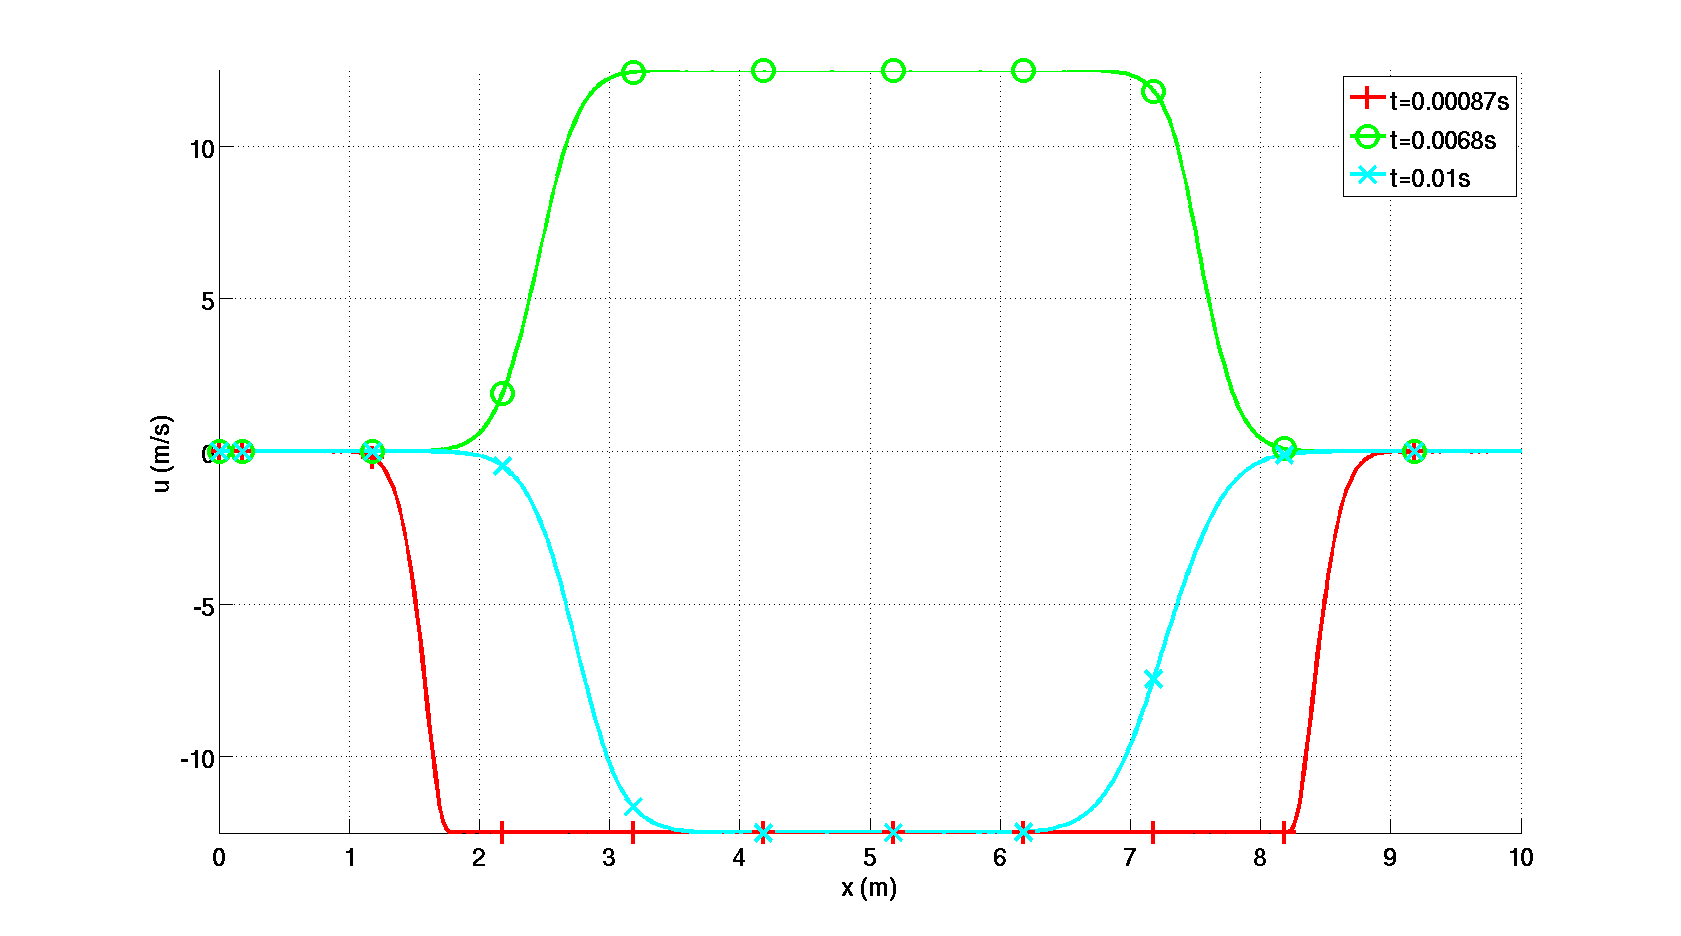
\includegraphics[width=\textwidth]{figures/Plot_velocity_single_phase.png}
                \caption{Velocity}
                \label{fig:single-phase-vel}
        \end{subfigure}%
        \begin{subfigure}[b]{0.5\textwidth}
                \centering
                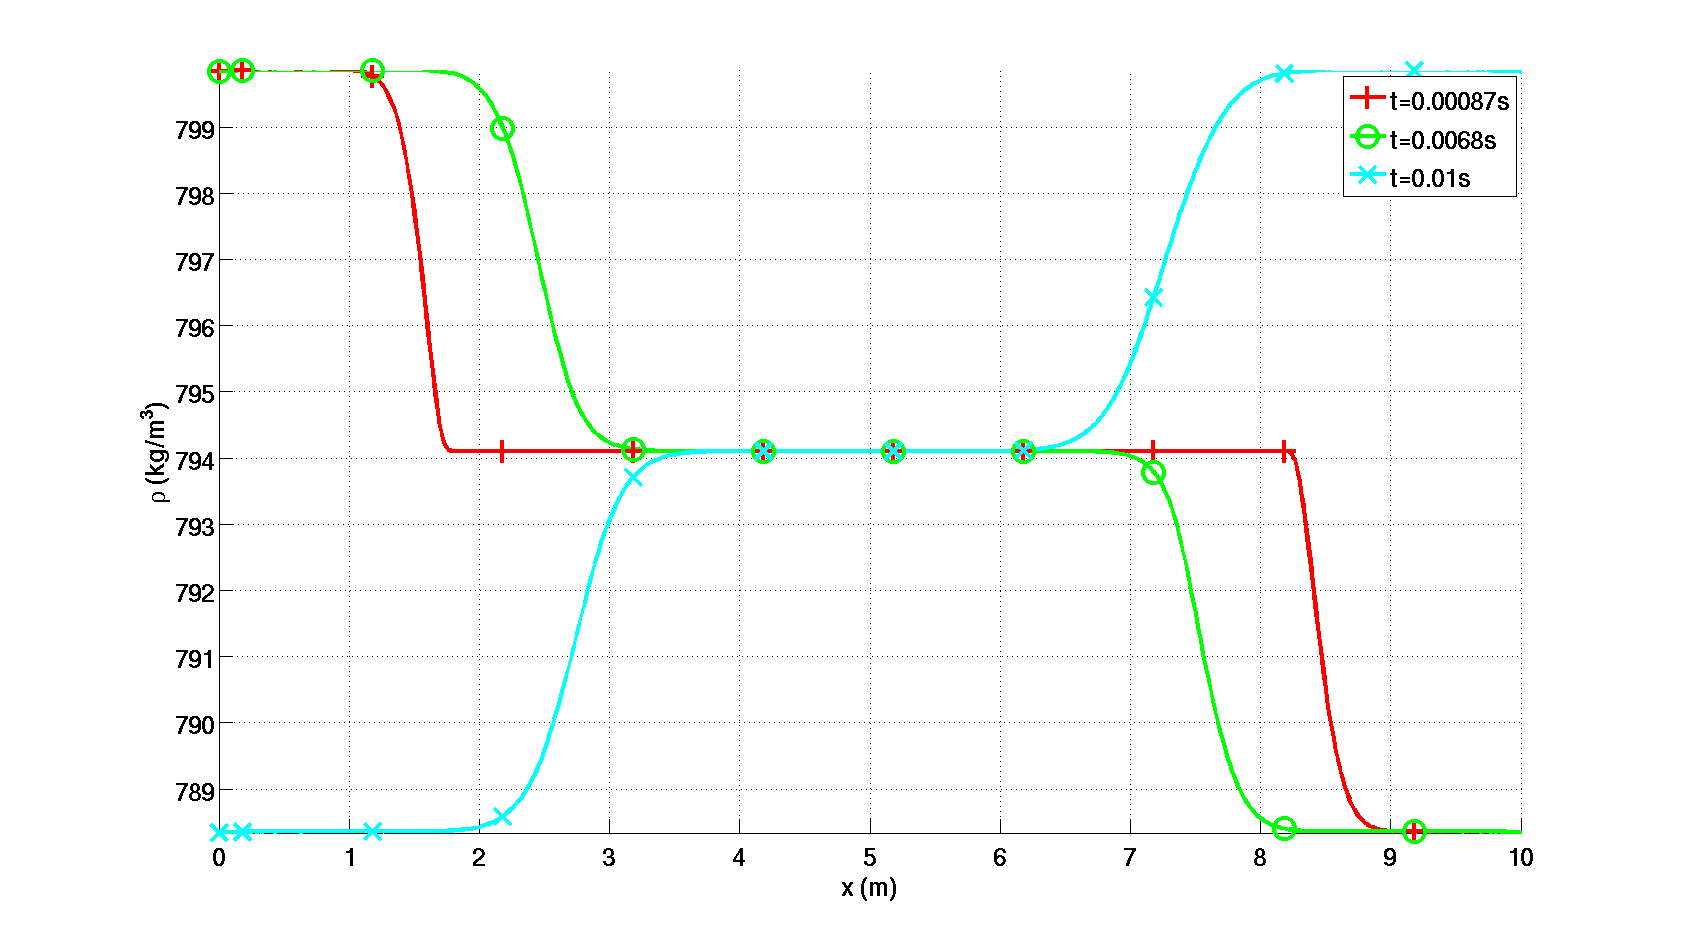
\includegraphics[width=\textwidth]{figures/Plot_density_single_phase.png}
                \caption{Density}
                \label{fig:single-phase-density}
        \end{subfigure}
        
        \begin{subfigure}[b]{0.495\textwidth}
                \centering
                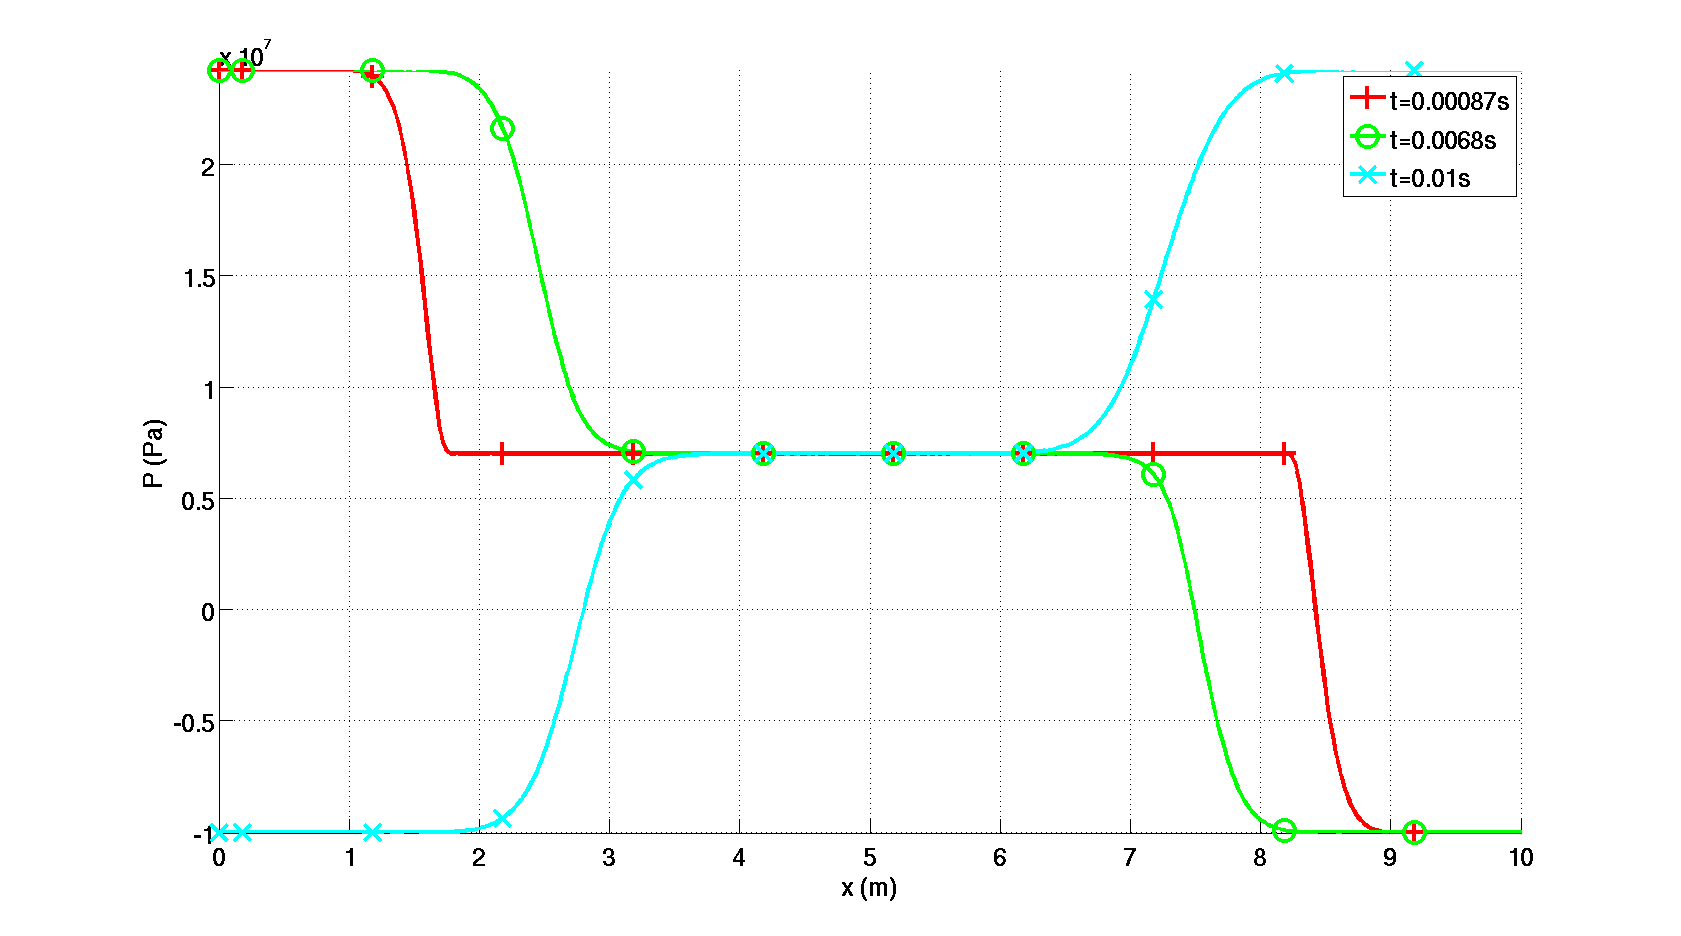
\includegraphics[width=\textwidth]{figures/Plot_pressure_single_phase.png}
                \caption{Pressure}
                \label{fig:single-phase-press}
        \end{subfigure}        
        \begin{subfigure}[b]{0.495\textwidth}
                \centering
                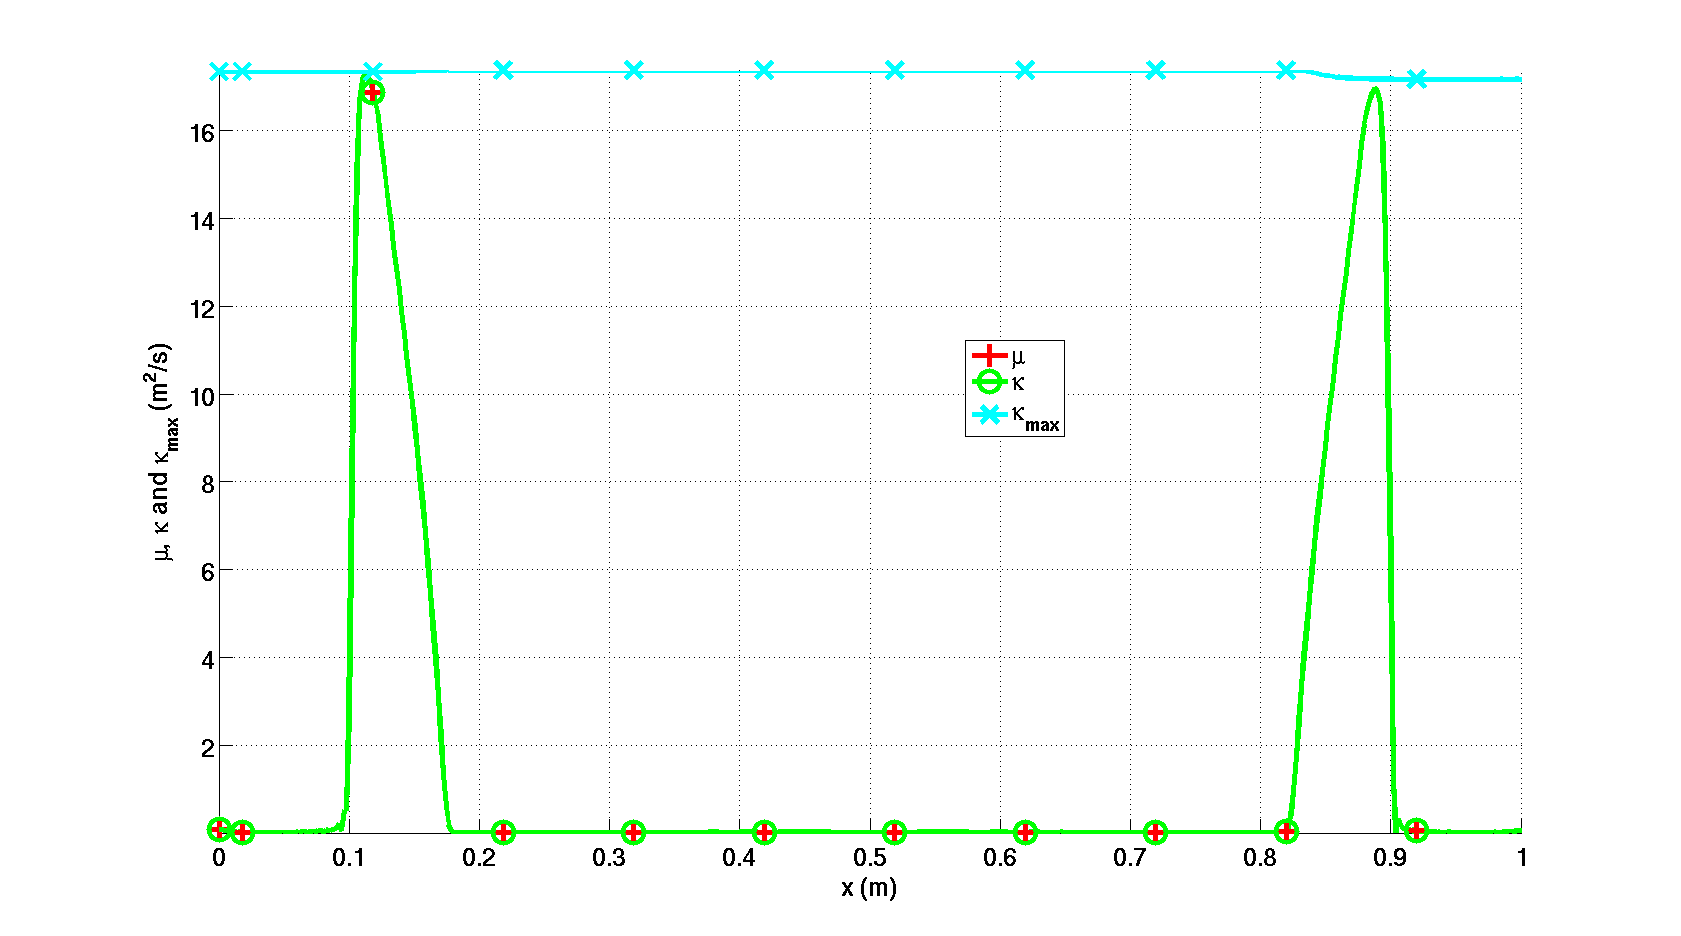
\includegraphics[width=\textwidth]{figures/Plot_viscosity_single_phase.png}
                \caption{Viscosity coefficients}
                \label{fig:single-phase-visc}
        \end{subfigure}
        \caption{Numerical solutions of a water hammer at times $t=8.7 \times 10^{-4}, \, 6.8 \times 10^{-3} \text{ and } 10^{-3}$ s (the viscosity coefficients are only shown at time $t=8.7 \times 10^{-4}$ s).}\label{fig:single-phase}
\end{figure}
%
In \fig{fig:single-phase}, the numerical solution does not display any oscillations or any spurious instabilities due to the numerics. The viscosity coefficients $\kappa$ and $\mu$ only saturate to the first-order viscosity coefficients, $\kappa_{max}$, around $x=0.1$ m and $x=0.9$ m which match the positions of the shocks waves at $t=8.7 \times 10^{-4}$. It is also noted that the accuracy of the shock wave decreases over time: the numerical dissipation comes from the temporal integrator and the large number of time steps ($1500$ time steps are used to reach $t=6.8 \times 10^{-3}$). The accuracy of the numerical solution could be improved over time by using a higher-order temporal integrator.% other than BDF2.
%
%---------------------------------------------------------------------------------------------------
\subsection{Two-phase flow water-hammer} \label{sec:two-num-res}
%---------------------------------------------------------------------------------------------------
%
The two-phase water hammer is identical to the single-phase water hammer described in \sct{sec:two-num-res}: the liquid and vapor phases have the same initial conditions and the liquid void fraction is initially set to $0.5$. The two phases are in interaction through the pressure and velocity relaxation terms (see \eqt{eq:sem-eq}) that are functions of the relaxation coefficients, $\mu_P$ and $\lambda_u$, computed with $A_{int} = 10^3$ $m^{-1}$ so that the two phases achieve pressure and velocity equilibrium at all times. Plots of the velocity, the density, the pressure and the viscosity coefficients are given in \fig{fig:liquid-phase} and \ref{fig:vapor-phase} for the liquid and gas phases, respectively.
%
\begin{figure}[H]
        \centering
        \begin{subfigure}[b]{0.5\textwidth}
                \centering
                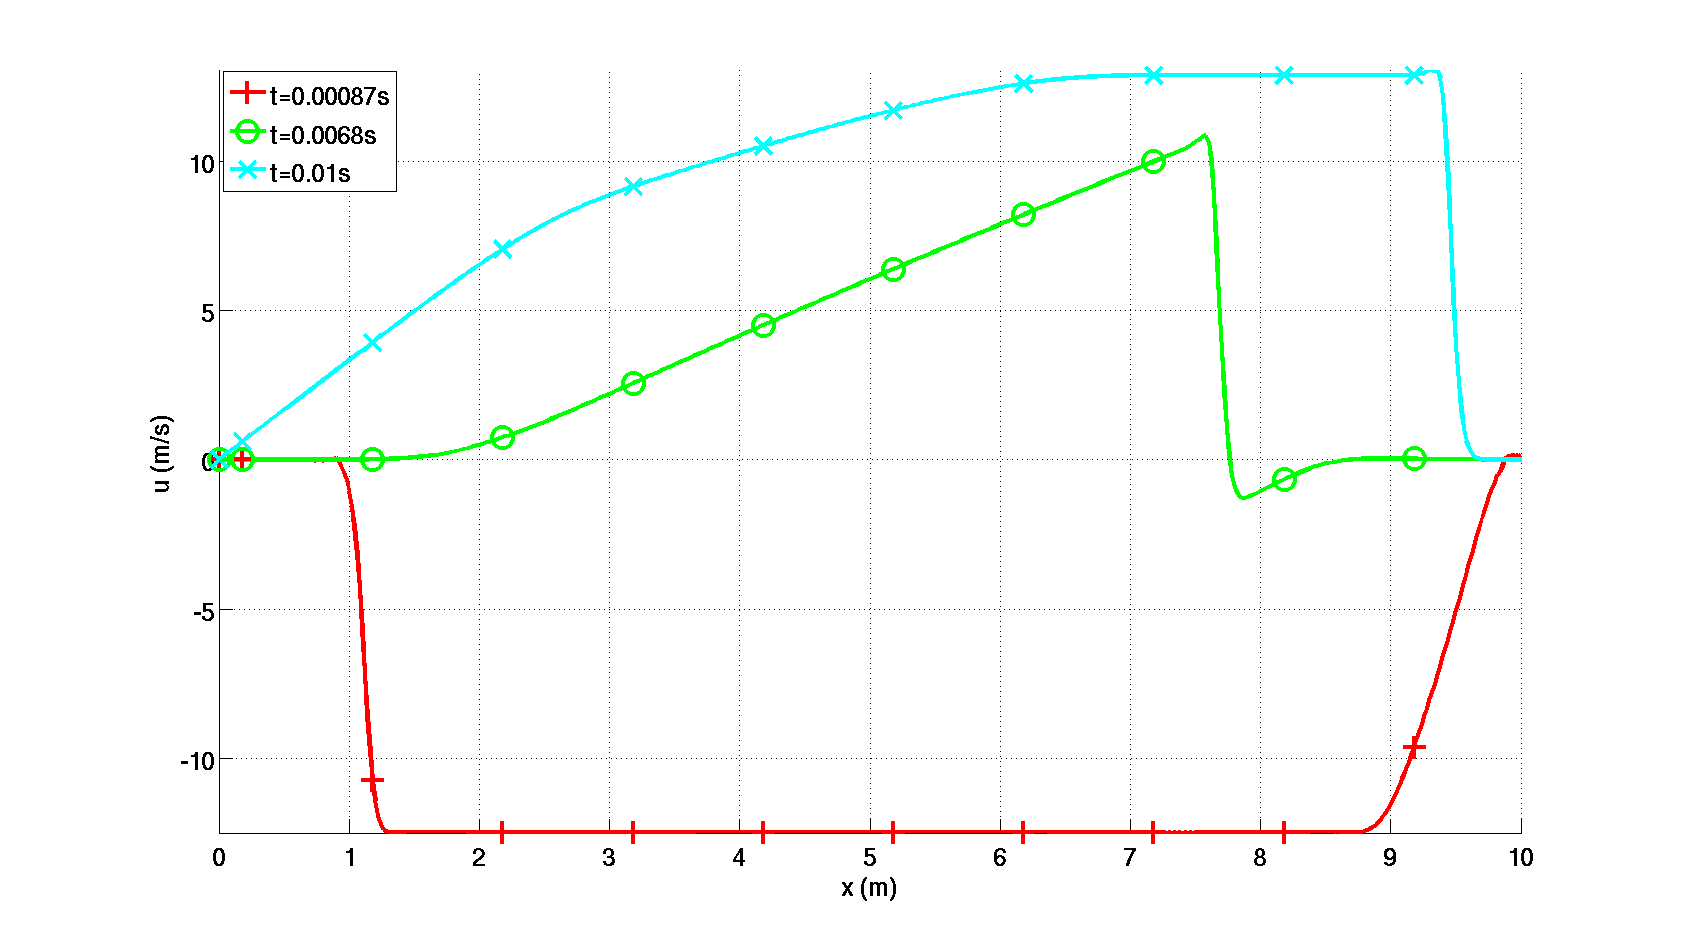
\includegraphics[width=\textwidth]{figures/Plot_velocity_liquid_phase.png}
                \caption{Liquid velocity}
                \label{fig:liq-phase-vel}
        \end{subfigure}%
        \begin{subfigure}[b]{0.5\textwidth}
                \centering
                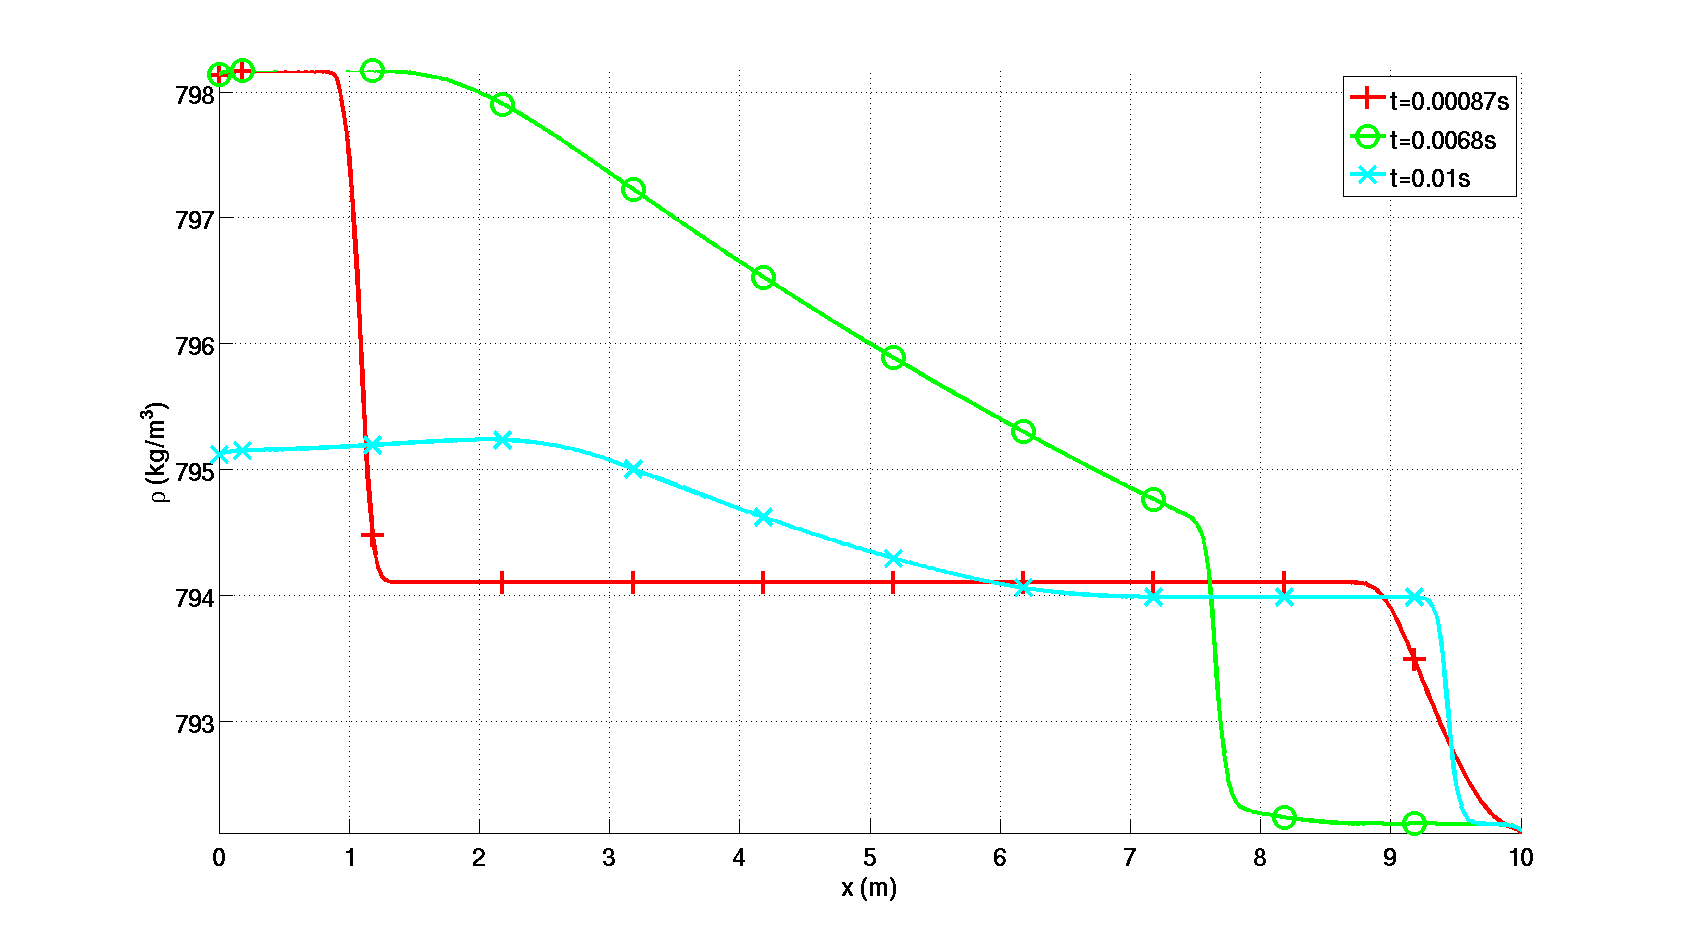
\includegraphics[width=\textwidth]{figures/Plot_density_liquid_phase.png}
                \caption{Liquid density}
                \label{fig:liq-phase-density}
        \end{subfigure}
        
        \begin{subfigure}[b]{0.495\textwidth}
                \centering
                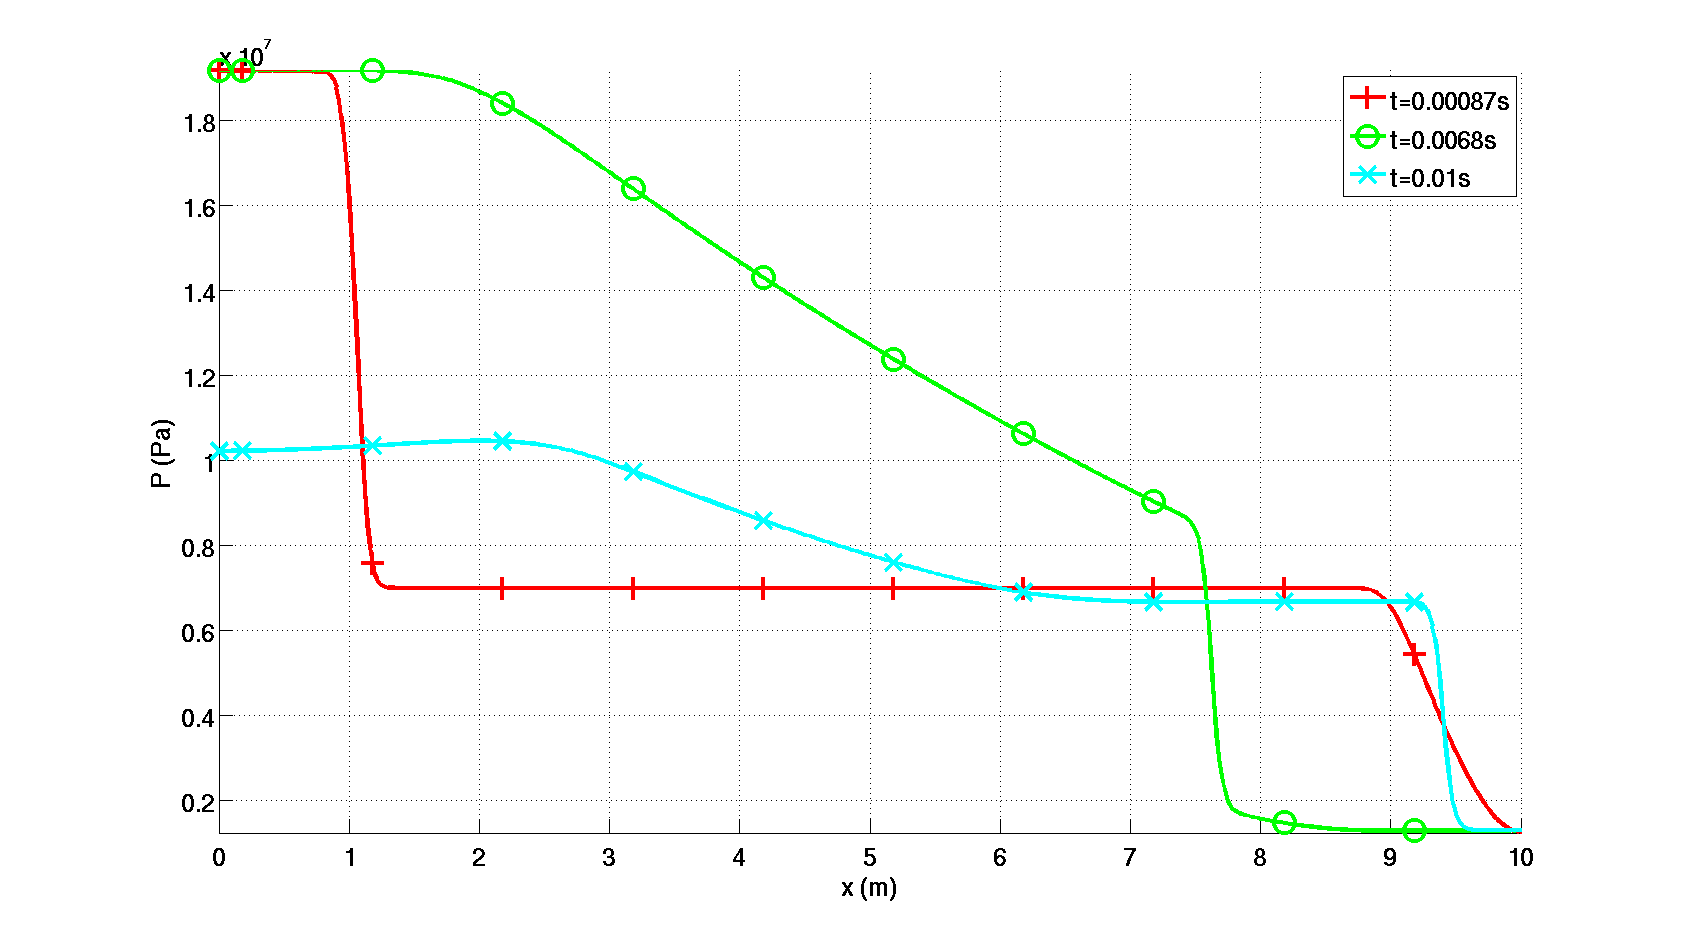
\includegraphics[width=\textwidth]{figures/Plot_pressure_liquid_phase.png}
                \caption{Liquid pressure}
                \label{fig:liq-phase-press}
        \end{subfigure}        
        \begin{subfigure}[b]{0.495\textwidth}
                \centering
                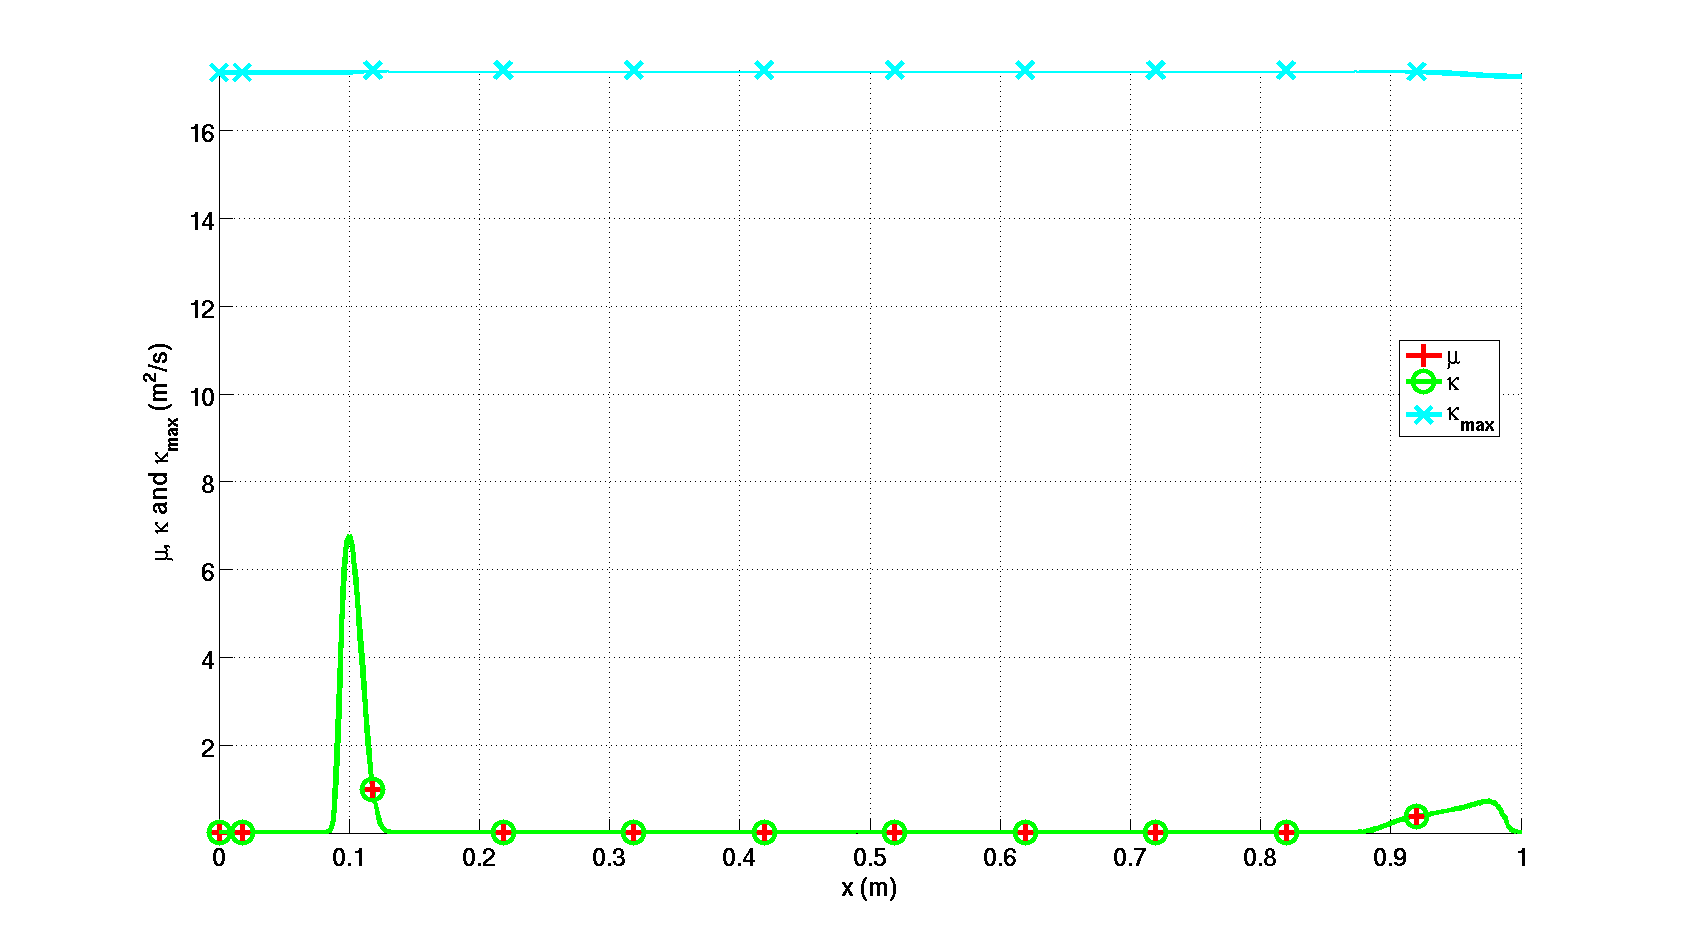
\includegraphics[width=\textwidth]{figures/Plot_viscosity_liquid_phase.png}
                \caption{Liquid viscosity coefficients}
                \label{ffig:liq-phase-visc}
        \end{subfigure}
        \caption{Numerical solutions for the liquid phase of a two-phase water hammer at times $t=8.7 \times 10^{-4}, \, 6.8 \times 10^{-3} \text{ and } 10^{-3}$ s (the viscosity coefficients are only shown at time $t=8.7 \times 10^{-4}$ s).}\label{fig:liquid-phase}
\end{figure}
%
%
\begin{figure}[H]
        \centering
        \begin{subfigure}[b]{0.5\textwidth}
                \centering
                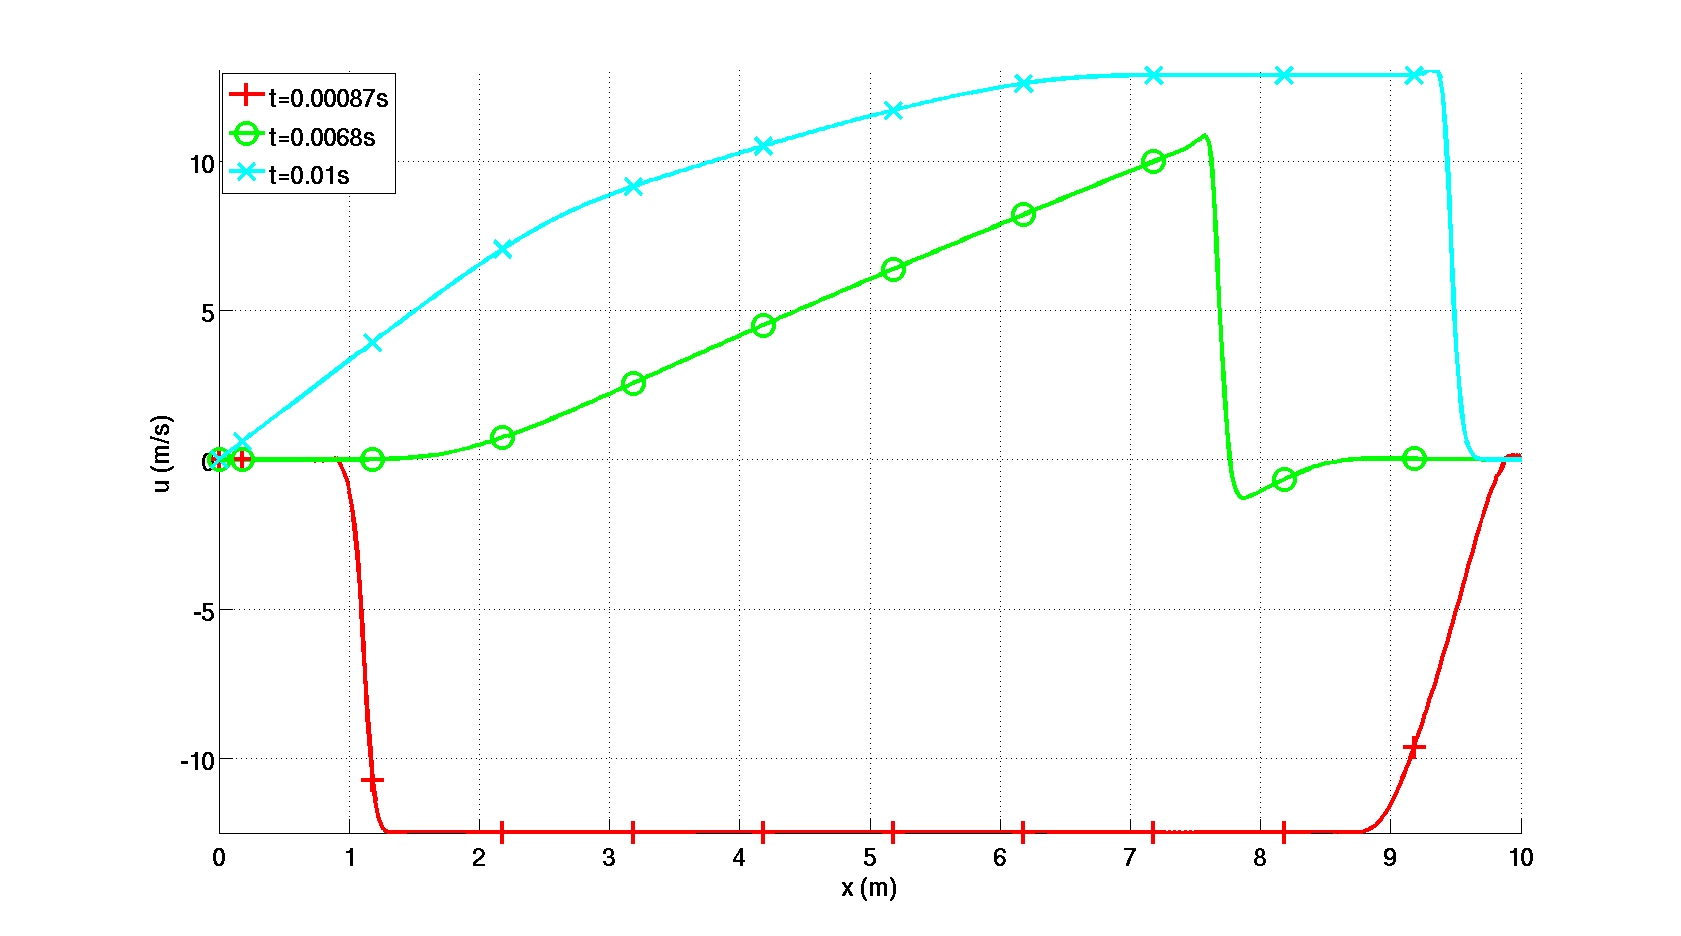
\includegraphics[width=\textwidth]{figures/Plot_velocity_gas_phase.png}
                \caption{Gas velocity}
                \label{fig:vap-phase-vel}
        \end{subfigure}%
        \begin{subfigure}[b]{0.5\textwidth}
                \centering
                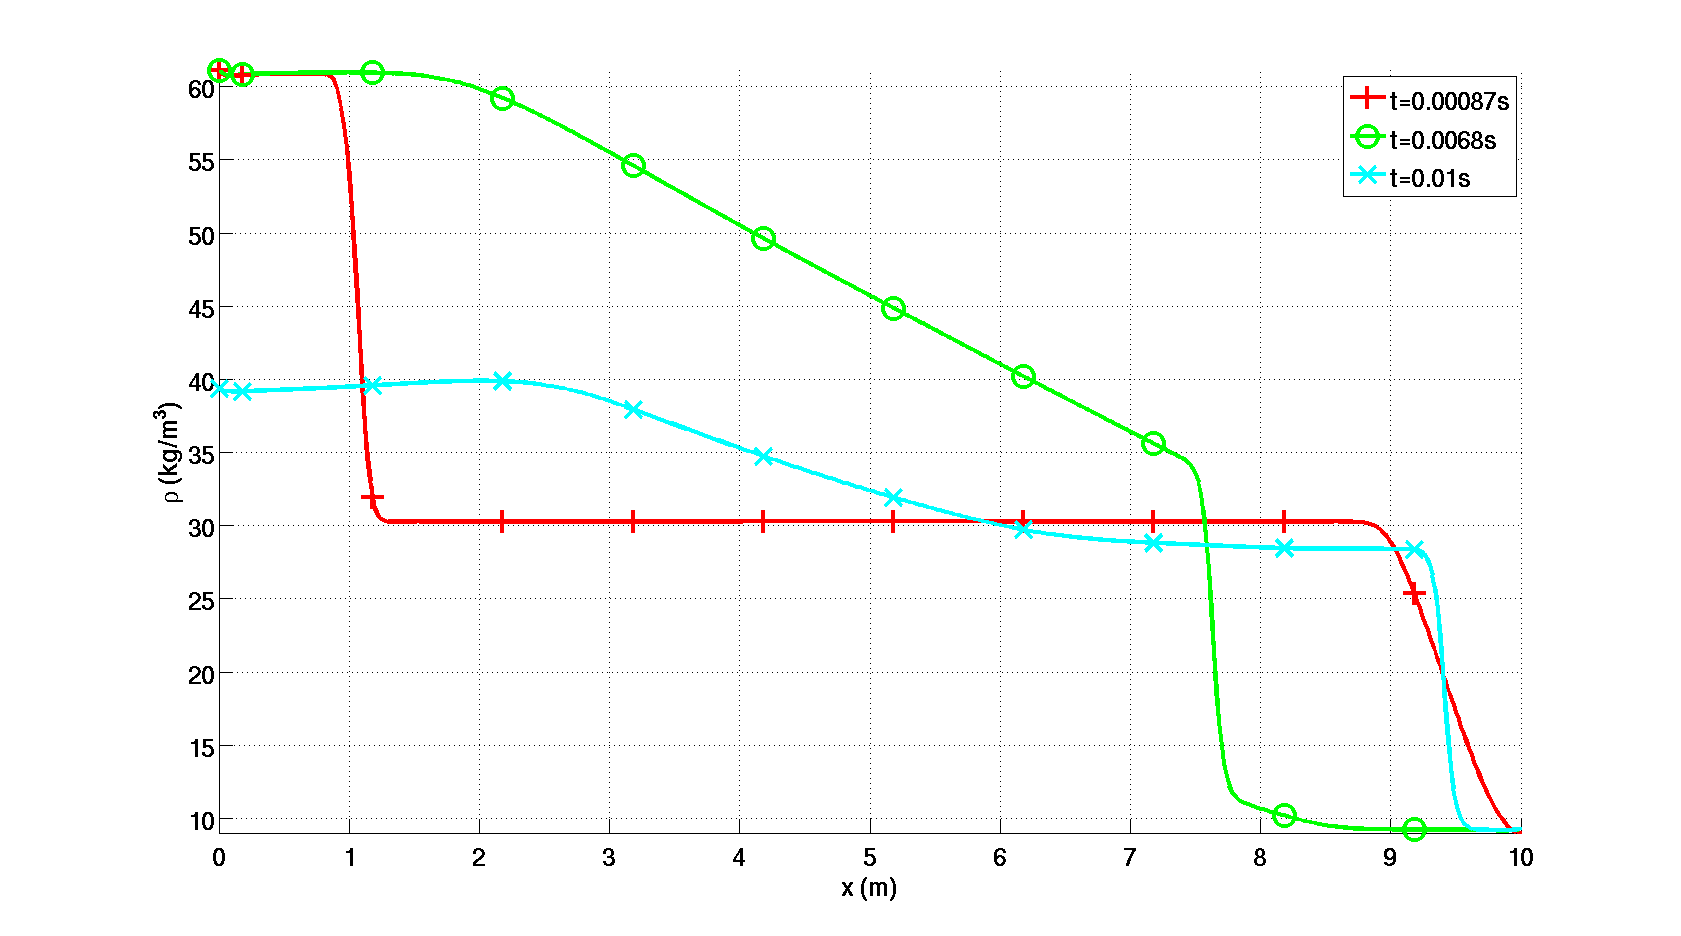
\includegraphics[width=\textwidth]{figures/Plot_density_gas_phase.png}
                \caption{Gas density}
                \label{fig:vap-phase-density}
        \end{subfigure}
        
        \begin{subfigure}[b]{0.495\textwidth}
                \centering
                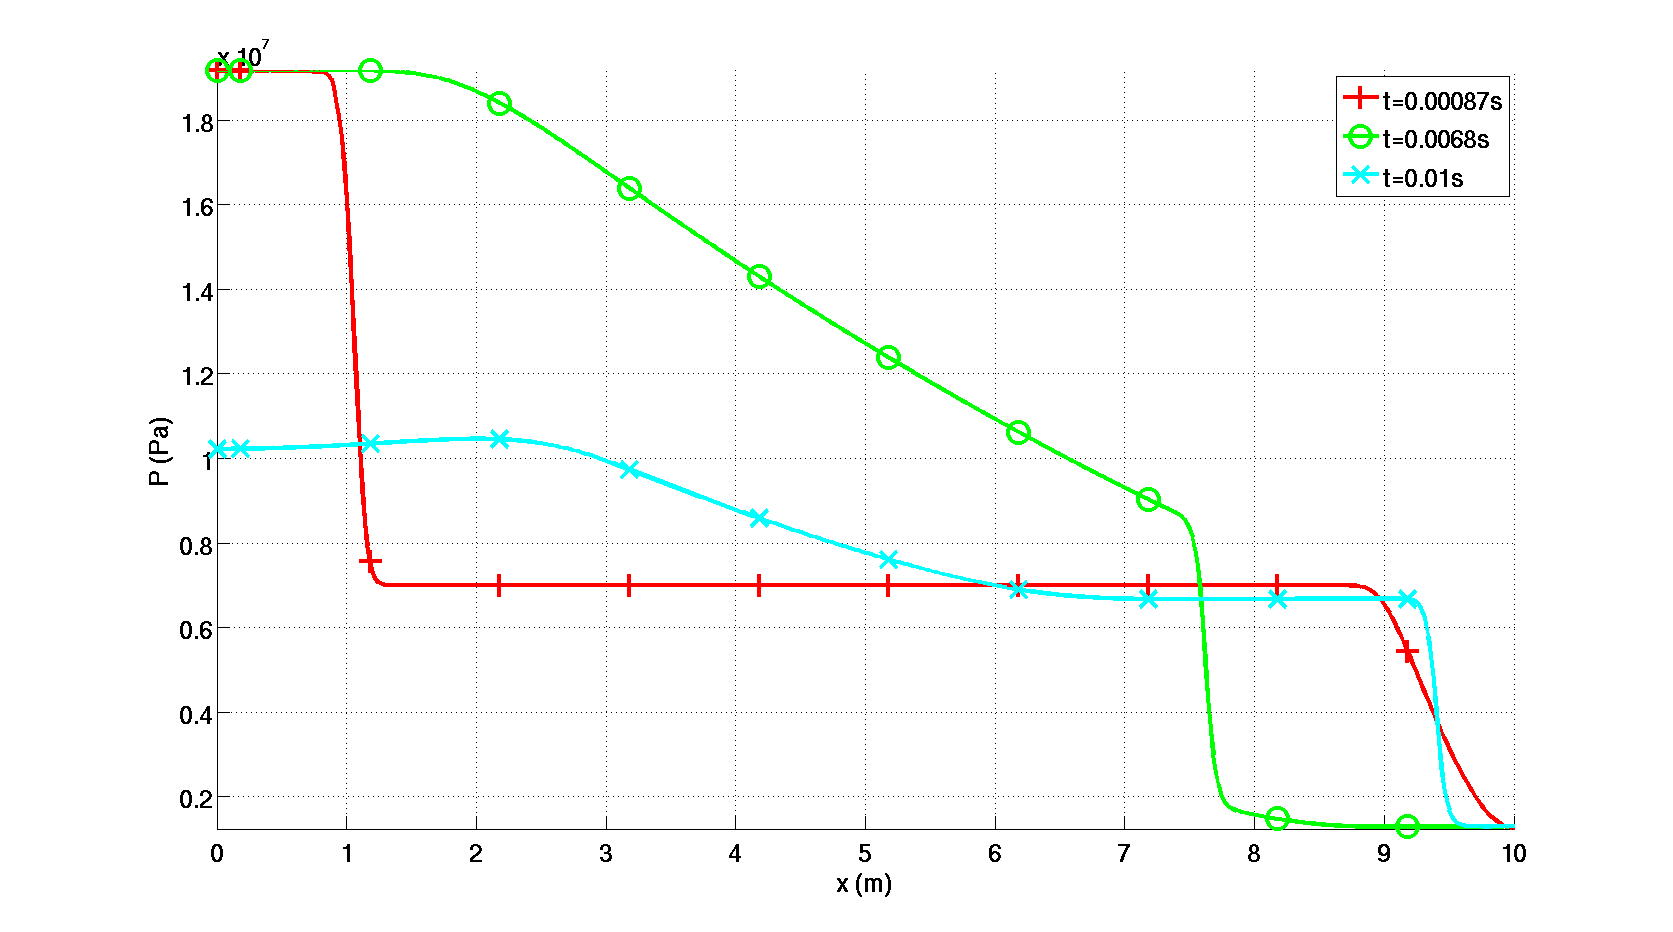
\includegraphics[width=\textwidth]{figures/Plot_pressure_gas_phase.png}
                \caption{Gas pressure}
                \label{fig:vap-phase-press}
        \end{subfigure}        
        \begin{subfigure}[b]{0.495\textwidth}
                \centering
                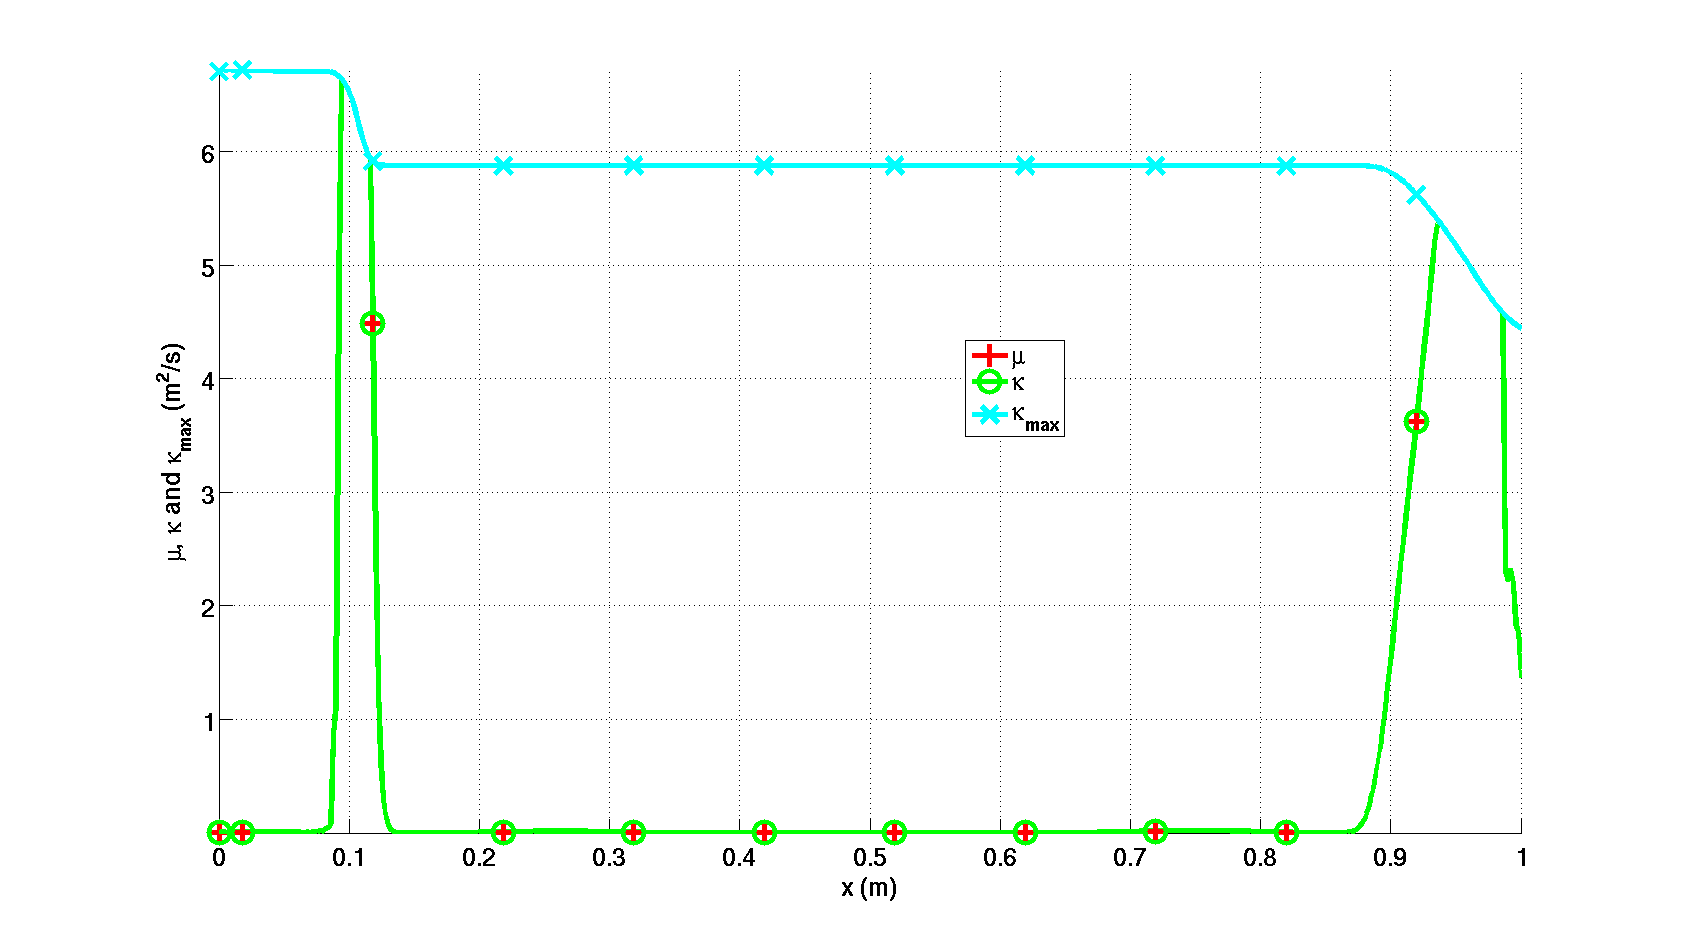
\includegraphics[width=\textwidth]{figures/Plot_viscosity_gas_phase.png}
                \caption{Gas viscosity coefficients}
                \label{fig:vap-phase-visc}
        \end{subfigure}
        \caption{Numerical solutions for the vapor phase of a two-phase water hammer at times $t=8.7 \times 10^{-4}, \, 6.8 \times 10^{-3} \text{ and } 10^{-3}$ s (the viscosity coefficients are only shown at time $t=8.7 \times 10^{-4}$ s).}\label{fig:vapor-phase}
\end{figure}
%
\fig{fig:liquid-phase} and ~\ref{fig:vapor-phase} show that the numerical solution of the liquid and gas phases do not display any oscillations or instabilities. 
As expected, the two fluids have the same pressure and velocity profiles as shown in \fig{fig:vap-phase-press}, ~\ref{fig:liq-phase-press} and \fig{fig:vap-phase-vel}, ~\ref{fig:liq-phase-press}, respectively. The shocks coming from the left and right walls are initially well resolved and do not display any instability but lose stiffness over time for the same reason as detailed in \sct{sec:single-num-res}. The density of the liquid and gas phases have different values but experience similar variations. The viscosity coefficients are plotted at time $t = 8.7 \times 10^{-3}$ s and display two peaks that match the shock positions.
%
%%%%%%%%%%%%%%%%%%%%%%%%%%%%%%%%%%%%%%%%%%%%%%%%%%%%%%%%%%%%%%%%%%%%%%%%%%%%%
%%%%%%%%%%%%%%%%%%%%%%%%%%%%%%%%%%%%%%%%%%%%%%%%%%%%%%%%%%%%%%%%%%%%%%%%%%%%%
\section{Conclusions and future work}\label{sec:conclusion}
%%%%%%%%%%%%%%%%%%%%%%%%%%%%%%%%%%%%%%%%%%%%%%%%%%%%%%%%%%%%%%%%%%%%%%%%%%%%%
%%%%%%%%%%%%%%%%%%%%%%%%%%%%%%%%%%%%%%%%%%%%%%%%%%%%%%%%%%%%%%%%%%%%%%%%%%%%%
%
We have presented numerical results of single- and a two-phase water hammers obtained with the system code RELAP-7. The numerical results show that the Entropy Viscosity Method is capable of stabilizing the schemes and that the viscosity coefficients are well-scaled. This work contributes to the assessment of the stabilization techniques for reactor flow problems computed with RELAP-7.

%%%%%%%%%%%%%%%%%%%%%%%%%%%%%%%%%%%%%%%%%%%%%%%%%%%%%%%%%%%%%%%%%%%%%
\section{Acknowledgments}

The research was carried out under the auspices of the Idaho National Laboratory for the US Department of Energy.

%%%%%%%%%%%%%%%%%%%%%%%%%%%%%%%%%%%%%%%%%%%%%%%%%%%%%%%%%%%%%%%%%%%%%
\setlength{\baselineskip}{12pt}

\bibliographystyle{mc2015}
\bibliography{mybibfile}



\end{document}
